\section{Otimização da Colônia de Formigas}

Na busca por alimento, as formigas utilizam de feromônios para encontrar o melhor caminho.
Isso acontece da seguinte maneira: cada formiga deposita feromônio ao se deslocar. A partir
da avaliação da quantidade de feromônio depositada por formigas que já passaram pelo local,
formigas subsequentes tem mais probabilidade de se mover em rotas que tem mais feromônios. Ao
decorrer do tempo os feromônios vão evaporando, apagando rastros que não foram reforçados. 
Com isso, caminhos que são percorridos por mais formigas tem mais chance de serem 
percorridos por outras formigas do que aqueles que foram percorridos por menos formigas e 
caminhos que foram percorridos á pouco tempo tem mais chance de serem percorridos que caminhos
percorridos a muito tempo. A quantidade de feromônio depositado é mais intensa no trajeto de volta,
quando a comida foi encontrada. Outro fator que é levado em consideração é a qualidade da comida
encontrada, de maneira que mais feromônio é depositado quanto melhor for a fonte de alimento encontrada.
A medida que mais formigas exploram o local e encontram alimento, esse procedimento tende a otimizar o
trajeto entre a fonte de alimento e a colônia.

Apesar dessa heurística utilizada pelas formigas ser interessante para se resolver problemas combinatórios 
do tipo NP(i.e., com complexidade não polinomial), são necessários algumas adaptações na construção
de um algoritmo computacional.

A seguir é apresentado a meta-heurística do ACO (\textit{Ant Colony Optimization}) algoritmo,
juntamente com observações relacionadas as diferenças entre a heurística do ACO e o
comportamento natural das formigas descrito anteriormente.

\subsection{Meta-heurística do ACO}

\begin{figure}[ht]
  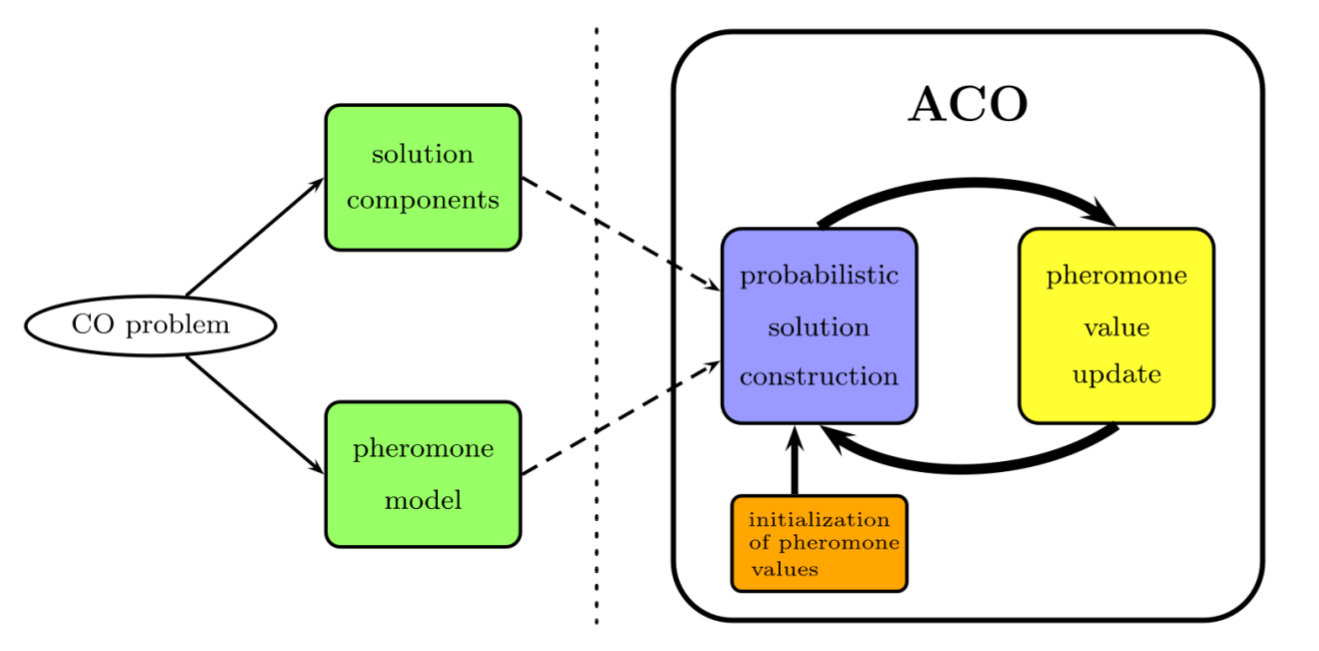
\includegraphics[width = 0.9 \linewidth]{imgs/meta_heuristica_aco}
  \label{diagrama_metaheuristica_aco}
  \caption{Diagrama de funcionamento da meta-heurística do ACO \cite{blum2005aco}}
\end{figure}

%Algoritmo
\begin{algorithm}[H]
  %Macros
  \SetKwBlock{AgendarAtividade}{AgendarAtividade}{fim}
  \SetKwBlock{Procedimento}{Procedimento}{fim}

  \Procedimento{
    \Enqto{$n < N_{MAX\_IT}$}{
      %\tcp*[f]{$N_{MAX\_IT}$ é o número máximo de iterações\\}
      \AgendarAtividade{
        ConstruirSolucoesFormigas\\
        AtualizarFeromonios\\
        %\tcp*[f]{opcional}\\
        \tcp{opcional:}
        AcoesGlobais
      }
    }
  }

  \caption{Pseudo código da meta-heurística do ACO\label{lst:meta-heuristica_aco}}
\end{algorithm}

A meta-heurística do ACO pode ser subdividida em três partes,
conforme proposto por \cite{doringo2004ant}: \textit{ConstruirSolucoesFormigas},
\textit{AtualizarFeromonios} e \textit{AcoesGlobais}.

\textit{ConstruirSolucoesFormigas} gerencia a movimentação de uma colônia de formigas
em torno dos nós vizinhos. A escolha do próximo nó é feita através de uma decisão
estocástica que é função da quantidade de feromônio no nós vizinhos e informação heurística.
Quando uma formiga encontra uma solução, ou enquanto a solução é construída, esta avalia a
qualidade da solução (completa ou parcial) que será utilizada pelo procedimento
\textit{AtualizarFeromonios} para decidir a quantidade de feromônio que será depositada.
Outro procedimento relevante na construção da solução é a eliminação de possíveis ciclos, utilizado
por exemplo, no problema do caixeiro viajante.

\textit{AtualizarFeromonios} é o processo que atualiza os traços de feromônio depositados pelas
formigas no espaço de busca. Os traços de feromônio podem aumentar, caso uma formiga tenha visitado
o nó/conexão em questão, ou diminuir, devido ao processo de evaporação do feromônio. Esse procedimento faz com 
que nós/conexões que foram visitados por muitas formigas ou por uma formiga e que tenha levado em
uma solução boa aumentem a probabilidade de serem visitados por futuras formigas. Semelhantemente, reduz 
a probabilidade de que nós que não foram visitados por novas formigas por muitas iterações sejam visitados
novamente. Logo, este procedimento evita a convergência a caminhos sub ótimos, favorecendo também a exploração
de novas regiões do espaço de busca.

Por fim, o procedimento \textit{AcoesGlobais} é utilizado para centralizar ações que não podem ser executadas
pelas formigas individualmente. Um exemplo de ações desse tipo é a filtragem de soluções ou o favorecimento de
regiões por meio de informações globais.

O procedimento \textit{AgendarAtividade} não necessariamente é uma instrução sequencial. Pode-se, portanto,
implementá-lo de maneira sequencial ou paralela, síncrona ou assincronamente. O tipo de abordagem que será
utilizada depende das características do problema que se deseja resolver.

\subsection{Exemplo de utilização}

\begin{figure}[ht]
  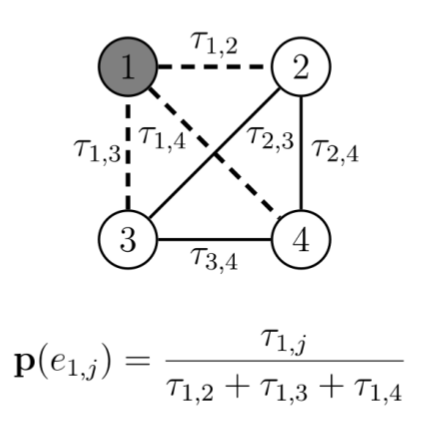
\includegraphics[width=0.32 \linewidth]{imgs/exemplo_aco_1}
  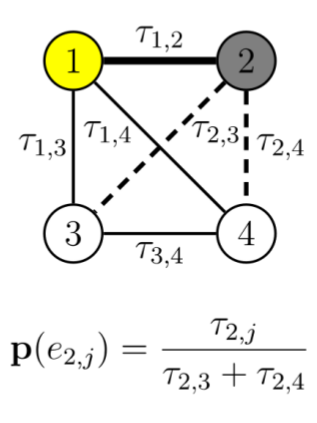
\includegraphics[width=0.32 \linewidth]{imgs/exemplo_aco_2}
  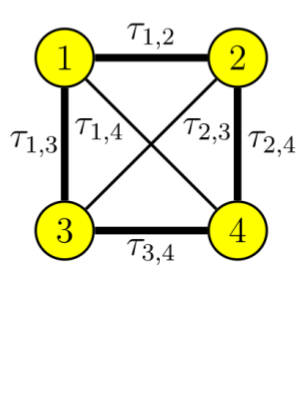
\includegraphics[width=0.32 \linewidth]{imgs/exemplo_aco_3}
  %\begin{subfigure}[b]
  %  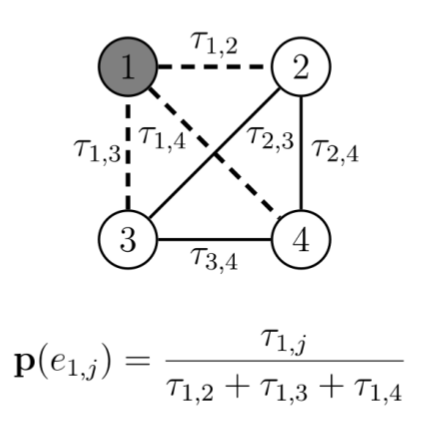
\includegraphics[width = 0.35 \linewidth]{imgs/exemplo_aco_1}
  %  \label{img:exemplo_aco_1}
  %\end{subfigure}
  %\begin{subfigure}
  %  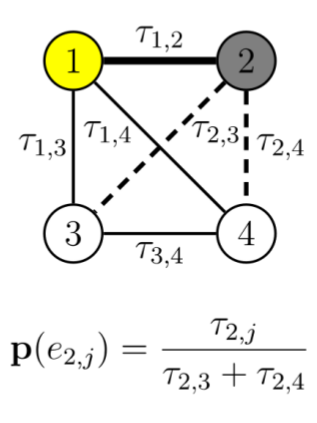
\includegraphics[width = 0.25 \linewidth]{imgs/exemplo_aco_2}
  %\end{subfigure}
  %\begin{subfigure}
  %  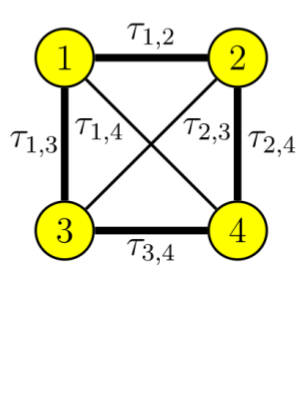
\includegraphics[width = 0.25 \linewidth]{imgs/exemplo_aco_3}
  %\end{subfigure}

  \label{img:exemp_aco}
  \caption{Example of the solution construction for a TSP problem}
  %It consists of 4 cities (modelled by a graph with 4 nodes; see Definition 1). The
  %solution construction starts by randomly choosing a start node for the ant;
  %in this case node 1. Figures (a) and (b) show the choices of the first,
  %respectively the second, construction step. Note that in both cases the
  %current node (i.e., location) of the ant is marked by dark gray color, and
  %the already visited nodes are marked by light gray color (respectively
  %yellow color, in the online version of this article). The choices of the ant
  %(i.e., the edges she may traverse) are marked by dashed lines. The probabilities
  %for the different choices (according to Eq. (4)) are given underneath the
  %graphics. Note that after the second construction step, in which we exemplary
  %assume the ant to have selected node 4, the ant can only move to node 3, and
  %then back to node 1 in order to close the tour. \cite{blum2005aco}}
\end{figure}

No TSP (\textit{Traveling Salesman Problem}) é dado um grafo completamente conectado e
não direcionado $G = (V , E)$ com pesos nas arestas.
Os nós $V$ do grafo representa as cidades e os pesos das arestas
distâncias entre as cidades. O objetivo é encontrar um caminho fechado em $G$
que contenha cada nó exatamente uma vez (portanto chamado passeio)
e cujo comprimento é mínimo. Logo, o espaço de busca $S$ consiste de todos os
passeios em $G$. O valor da função objetivo $f(s)$ de um passeio $s \in S$ 
é definido pela soma dos pesos das arestas que existem em $s$. O TSP pode ser
modelado de diverças maneiras como um problema de otimização discreta.
O modelo mais comum consiste de uma variavel binária de decisão $X_e$ para
cada aresta em $G$.
Se em uma solução $X_e = 1$, então a aresta $e$ participa do passeio definido pela solução.

No que se refere abordagem do TSP usando ACO, 
as arestas de um dado grafo do TSP podem ser consideradas componentes da solução,
i.e., para cada $e_{i,j}$ é introduzido um valor de feromônio $\tau_{i,j}$. 
A tarefa de cada formiga consiste em construir uma solução plausível para o TSP, i.e,
um passeio realizável. Em outras palavras, a noção de uma tarefa para uma formiga
muda de \textit{“escolher um caminho da colônia à fonte de comida”} para \textit{“
construir uma possível solução para o problema de otimização abordado"}. Note que com essa
mudança de tarefa, as noções de colônia e fonte de comida perdem seu significado.

Cada formiga constroe uma solução da seguinte maneira.
Primeramente, um dos nós do grafo do TSP é aleatóriamente selecionada como sendo nó inicial.
Então, cada formiga constroe seu passeio no grafo do TSP movendo-se em cada iteração de construção
de seu nó atual (i.e., a cidade na qual ela esta localizada) á outro nó que ela ainda não visitou.
A cada passo (iteração) a aresta percorrida é adicionada a solução em construção. Quando não 
restam nenhum nó não-visitado a formiga fecha o passeio movendo-se de seu nó atual até
o nó inicial, selecionado aleatoriamente no início da construção da solução. Dessa maneira a 
construção da solução implica que a formiga tem memória $T$ para armazenar os nó já
visitados. Cada iteração da solução é executado da seguinte maneira. 
Assumindo que a formiga esteja no nó $v_i$ , a subsequente iteração de solução é executada com probabilidade:

\begin{equation}
  \emph{p}(e_{i,j}) = \frac{\tau_{i,j}}{\sum_{k \in \lbrace 1,...,
  \vert V \vert\rbrace, v_k \not\in T}\tau_{i,k}},
  \forall j \in \lbrace 1,...,\vert V \vert\rbrace, v_j \not\in T
\end{equation}

Para um exemplo de tal construção de solução  veja Fig. \ref{img:exemp_aco}.
Uma vez que todas as formigas de colônia tenham completado a construção de sua
solução, a evaporação do feromônio é executada da seguinte maneira:

\begin{equation}
  \tau_{i,j} \leftarrow (1-\rho)\cdot \tau_{i,j}, \forall \tau_{i,j}\in \mathcal{T}
\end{equation}

Onde $\mathcal{T }$ é o conjunto de todos os valores de feromônio.
Então as formigas executam seu respectivos passeios. Dessa maneira,
para cada $e_{i,j} \in s$ o seguinte feromônio é depositado:

\begin{equation}
  \tau_{i,j} \leftarrow \tau_{i,j} + \frac{Q}{f(s)}
\end{equation}

Onde $Q$ é novamente uma constante positiva e $f(s)$ é o valor da função objetivo
da solução $s$. O sistema esta iterativamente aplicando $n_a$ 
formigas por iteração até que condição de parada
(e.g., o tempo limite) seja satisfeita.
Mesmo que o \textit{AS algorithm} tenha provado que o comportamento das formigas
descrito anteriormente (no inicio da seção) pode ser tranferido para um algorítmo 
de otimização discreta, foi
em geral descoberto que ele é inferior aos algoŕtmos do estado da arte.
Portanto, ao longo dos anos várias extensões e aprimoramentos do algorítimo
original de resolução do TSP usando ACO foram introduzidas. Todos eles combrem a definição de metaheurística do ACO,
descrito anteriormente.
 
\subsection{Aplicação ao Problema}
